%============================================================================
% CHAPTER 2: LITERATURE REVIEW
% Institute of Technology of Cambodia
% Delta Robot Vision-Based Control System
% Academic Year: 2025-2026
%============================================================================

\section{LITERATURE REVIEW}

\subsection{State-of-the-Art}
\hspace{1.27cm}
This chapter examines the body of knowledge underpinning the design and
implementation of the proposed system. Topics covered include the
historical development and kinematic theory of Delta robots, techniques
for vision-based localisation of objects in a robot workspace, deep
learning approaches to object detection, the mathematical basis for
transforming coordinates between camera and robot frames, and
software frameworks for real-time motion control. Several published
implementations of low-cost, vision-guided Delta robot systems are
also reviewed and compared to contextualise the contributions made in
this work.

%============================================================================
\subsubsection{History and Concept of Delta Robotics}
\hspace{1.27cm}
The Delta robot emerged from research conducted by Professor Reymond
Clavel at the \'{E}cole Polytechnique F\'{e}d\'{e}rale de Lausanne
(EPFL) in 1985, motivated by the need for a manipulator capable of
handling lightweight objects at speeds that conventional serial robots
could not achieve \autocite{clavel-1990}, as shown in
\textbf{\autoref{fig:first_delta_robot}}. The mechanism is built
around a parallel kinematic structure in which three mechanically
identical limbs connect a stationary base to a moving end-effector
platform. Each limb consists of a proximal arm driven directly by a
rotary actuator mounted on the base, and a distal forearm formed by a
passive parallelogram linkage. The geometric effect of these
parallelogram linkages is to restrict the platform to purely
translational movement, meaning the orientation of the end-effector
remains fixed regardless of where within the workspace it is
positioned. This constraint yields exactly three translational degrees
of freedom (DOF).

\begin{figure}[h]
    \centering
    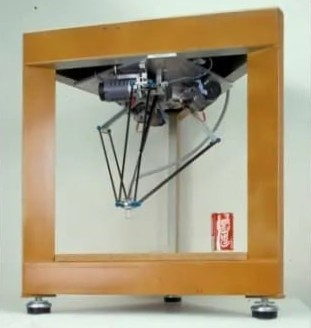
\includegraphics[width=0.55\linewidth]{image/first_delta_robot.jpg}
    \caption{The First Delta Robot Prototype Developed by Professor
             Reymond Clavel at the \'{E}cole Polytechnique
             F\'{e}d\'{e}rale de Lausanne (EPFL) in 1985
             \autocite{clavel-1990}.}
    \label{fig:first_delta_robot}
\end{figure}

\par
\hspace{1.27cm}
Because all three actuators are fixed to the stationary base, the
only mass in motion during operation is the lightweight platform
itself, which dramatically reduces the effective inertia of the system
and allows the mechanism to complete a full pick-and-place cycle in
under one second. Clavel formally documented the kinematic
architecture in U.S.\ Patent 4,976,582, and subsequent analyses by
researchers in the robotics community have validated and extended
the original kinematic formulations \autocite{merlet-2006,
stock-2003}. Industrially, this architecture has proven highly
successful: commercial variants produced by ABB (marketed as the
FlexPicker) and by Fanuc routinely achieve positional repeatability
figures of $\pm$0.1\,mm alongside cycle times shorter than
0.3\,seconds, establishing the Delta robot as the leading platform
for high-volume pick-and-place in food processing, pharmaceutical
packaging, and electronics manufacturing \autocite{pierrot-1991}.

%============================================================================
\subsubsection{Recent Research and Applications}
\hspace{1.27cm}
The three case studies reviewed below were chosen on the basis that
each shares key technical elements with the system developed in this
thesis, namely a vision-guided Delta robot, real-time object
detection, and a design approach oriented toward low manufacturing
cost.

\begin{itemize}
    \item \textbf{Case Study 1: Visual Servo Kinematic Control of
    Delta Robot Using YOLOv5 Algorithm.}\par
    \hspace{1.27cm}
    Among the works reviewed, this study bears the closest structural
    resemblance to the system proposed here. It establishes a
    continuous vision-to-motion pipeline that begins with YOLO-based
    object detection, proceeds through a hand-eye coordinate mapping
    stage, and terminates in analytical IK computation and motor
    activation, as illustrated in \textbf{\autoref{fig:case1_image}}.
    \autocite{yamtuan-2023} constructed their robot with proximal and
    distal arm lengths of 200\,mm and 500\,mm respectively, and
    selected three Yaskawa AC servo motors driven via an Arduino Due
    board as the actuation system. Under test conditions the platform
    achieved a maximum tracking velocity of 214.55\,mm/s and a
    worst-case positioning error of 1.36\,mm. Object positions were
    estimated purely in the horizontal plane from RGB image
    coordinates, treating the vertical pick height as a constant
    known value. A notable weakness of this implementation is that
    motor commands are issued through low-level PWM signals generated
    directly from the microcontroller, with no modular software layer
    separating the perception and motion subsystems.\par
    \hspace{1.27cm}
    The perception subsystem relied on a standard 30\,fps USB webcam
    capturing frames at $640 \times 480$\,pixels, with the YOLOv5
    detector integrated into a Python and OpenCV processing pipeline.
    Hand-eye calibration was performed by rotating the camera
    coordinate frame by $\beta = 150^{\circ}$ relative to the robot
    base frame and establishing a scale factor of 0.834\,mm/pixel
    through a linear regression procedure. During evaluation, the
    system successfully sorted eight medicine boxes of four different
    classes within 46\,seconds. Detection quality was assessed at a
    training mean average precision of 85\% and a validation score
    of 81\%, with spatial localisation errors remaining below
    3.5\,mm for unoccluded objects \autocite{yamtuan-2023}.\par
    \begin{figure}[h]
        \centering
        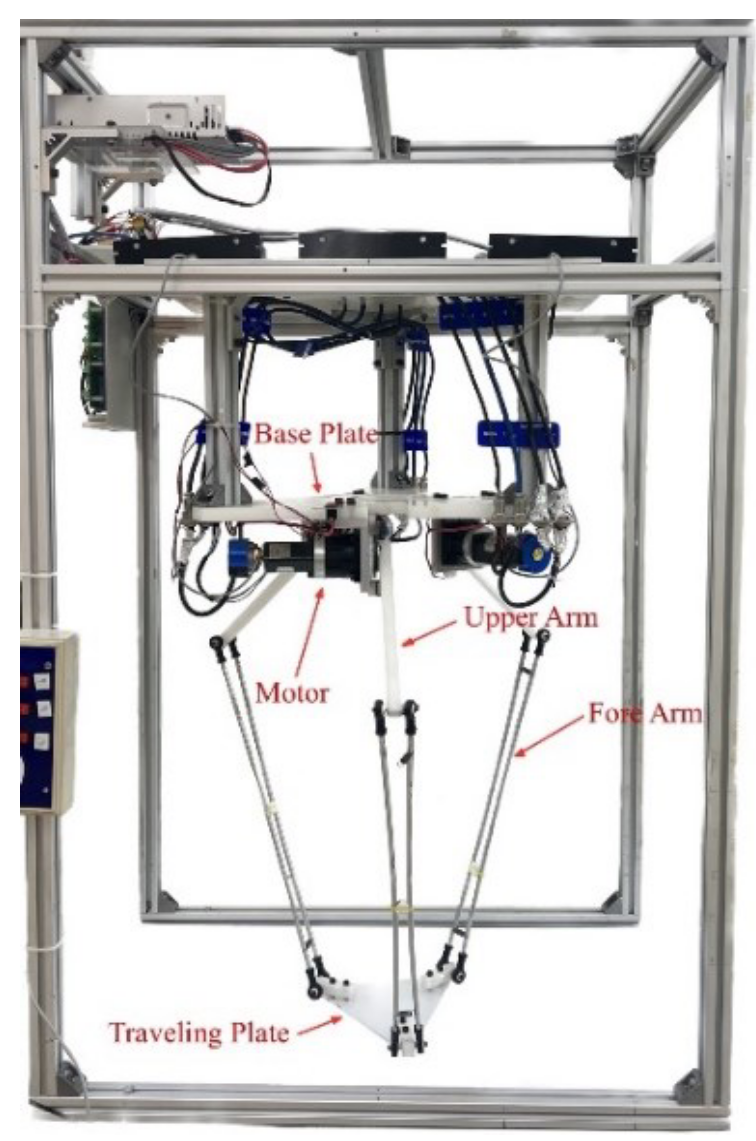
\includegraphics[width=0.4\linewidth]{image/Study Case 1.png}
        \caption{Delta robot platform employing YOLOv5-based visual
                 servoing for automated sorting of medicine boxes
                 \autocite{yamtuan-2023}.}
        \label{fig:case1_image}
    \end{figure}

    \item \textbf{Case Study 2: Design a Low-Cost Delta Robot Arm for
    Pick-and-Place Applications Based on Computer Vision.}\par
    \hspace{1.27cm}
    This work investigated the extent to which vision-based
    pick-and-place can be realised on a Delta robot built entirely
    from inexpensive, off-the-shelf parts \autocite{le-2023}. To
    minimise fabrication expense, the structural frame shown in
    \textbf{\autoref{fig:case2_image}} was produced through a
    combination of laser cutting and fused deposition modelling, a
    strategy that preserved adequate mechanical rigidity for
    bench-scale operation while avoiding the cost of machined
    components. Stepper motors replaced the servo actuators typical
    of higher-cost designs, and an Arduino Uno board was used as the
    central controller, accepting target coordinates and issuing the
    corresponding step sequences to each joint.\par
    \hspace{1.27cm}
    Object positions in the workspace were derived from images
    captured by a single fixed-overhead camera, eliminating the
    requirement for depth sensing hardware. Under the assumption that
    all target objects rest on a flat surface at a uniform, pre-measured
    height, the horizontal spatial coordinates could be back-calculated
    from the detected pixel location using the known camera geometry
    and pre-calibrated intrinsic parameters. An additional capability
    of this system was the estimation of object width from bounding
    box dimensions, which was used to set the gripper jaw separation
    dynamically before each grasp, enabling the robot to accommodate
    objects of different sizes within the same operational cycle.\par
    \hspace{1.27cm}
    Validation trials were carried out on three target objects
    differing in both geometry and dimensions. Across these trials the
    system demonstrated consistent detection, correct spatial
    estimation, and successful grasp-and-place sequences, supporting
    the conclusion that centimetre-level accuracy is attainable with
    monocular vision and low-cost mechanical hardware \autocite{le-2023}.\par
    \begin{figure}[h]
        \centering
        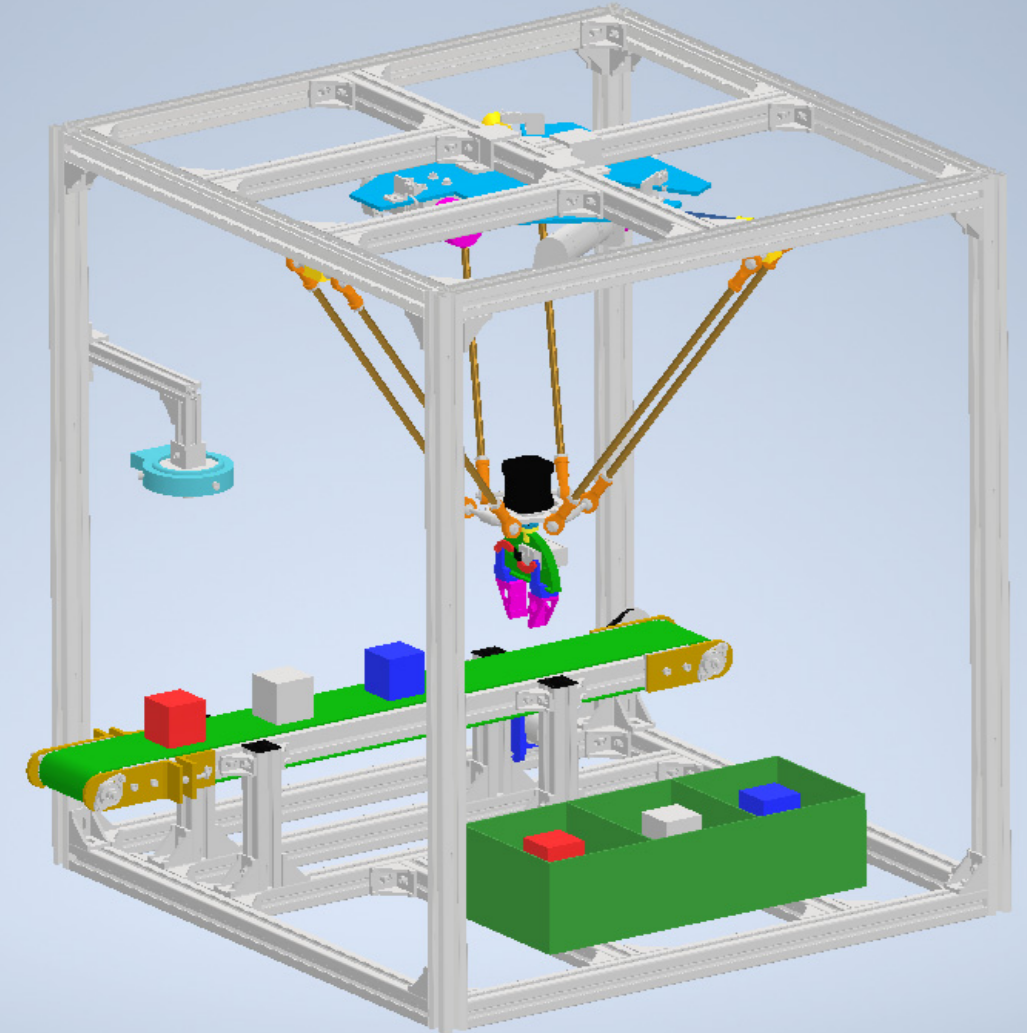
\includegraphics[width=0.5\linewidth]{image/Autodesk Study Case2.png}
        \caption{Low-cost Delta robot with monocular computer vision
                 for width-adaptive pick-and-place
                 \autocite{le-2023}.}
        \label{fig:case2_image}
    \end{figure}

    \item \textbf{Case Study 3: Low-Cost Parallel Delta Robot for a
    Pick-and-Place Application with the Support of the Vision
    System.}\par
    \hspace{1.27cm}
    Researchers at Benha University in Egypt constructed a
    fully operational Delta robot pick-and-place cell using
    components that are both inexpensive and readily obtainable
    \autocite{elassal-2024}. The mechanical frame was cut from
    aluminium alloy sheet using laser equipment, with joints
    produced by 3D printing. Three NEMA~17 stepper motors served
    as the actuators, each powered by a TB6600 driver operating
    at 24\,V and coordinated by an Arduino Mega~2560 controller.
    The mechanical geometry was characterised by a proximal arm
    length $L = 175$\,mm, a distal arm length $i = 330$\,mm, a
    fixed-plate radius $R = 150$\,mm, and a moving-platform
    radius $r = 111.4$\,mm. To map the reachable workspace,
    a MATLAB simulation swept each joint angle in 24 equal
    increments over the range $[-40^{\circ},\, 80^{\circ}]$.\par
    \hspace{1.27cm}
    A Raspberry Pi~3 Model~B+ acted as the master computing
    unit, executing a Python-based OpenCV vision pipeline that
    processed images from a Camera Module~V2 positioned above
    the conveyor. Target objects were identified through HSV
    colour segmentation combined with contour analysis, allowing
    classification by colour, shape, and approximate dimensions.
    Coordinate mapping from image pixels to robot base-frame
    positions was accomplished via a Least Squares Analysis (LSA)
    regression model that learned the linear relationship between
    pixel coordinates $(X_s,\, Y_s,\, Z_s)$ and robot-frame
    coordinates $(X_r,\, Y_r,\, Z_r)$ from a set of calibration
    measurements. Rather than synchronising robot motion with a
    continuously moving belt, the conveyor was halted temporarily
    by mechanical limit switches while the robot completed each
    pick cycle. The complete system was assembled for approximately
    800\,USD \autocite{elassal-2024}.\par
    \begin{figure}[h]
        \centering
        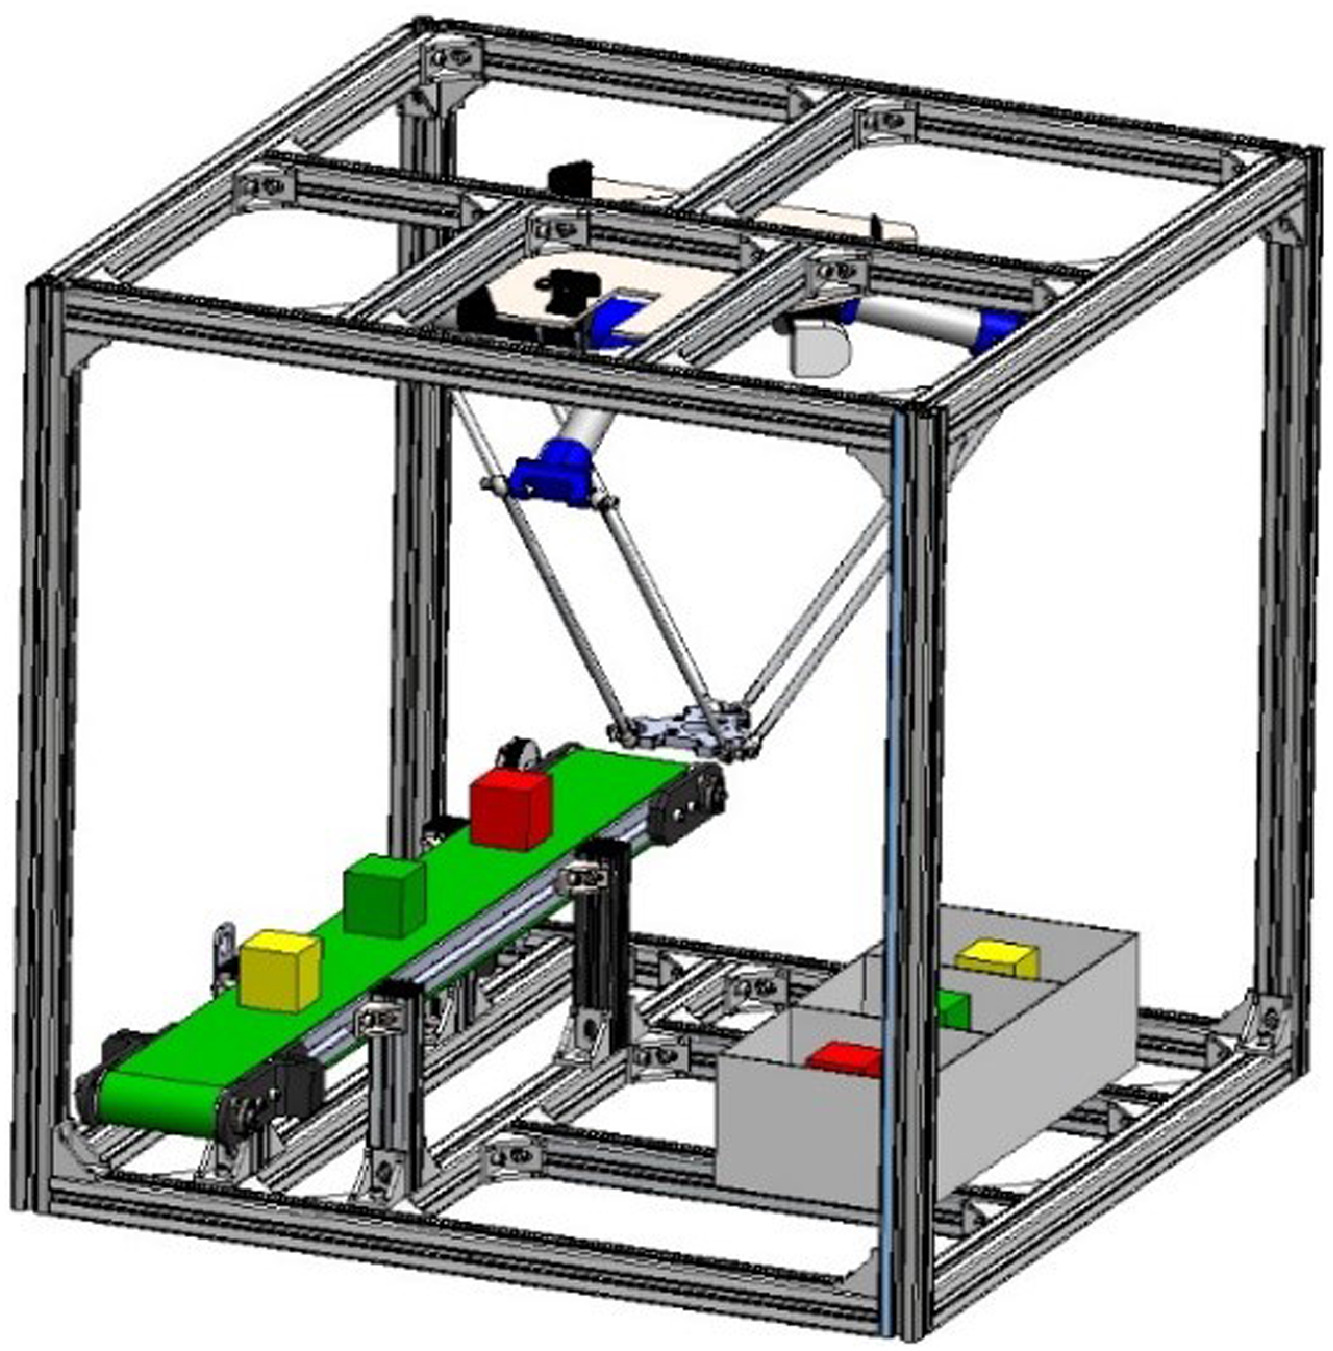
\includegraphics[width=0.5\linewidth]{image/Study Case 3.jpg}
        \caption{Low-cost Delta robot integrated with an HSV-based
                 colour vision system for conveyor-based sorting
                 \autocite{elassal-2024}.}
        \label{fig:case3_image}
    \end{figure}
\end{itemize}

%============================================================================
\subsection{Robot Manipulator}
\hspace{1.27cm}
A robot manipulator is a programmable mechanical system designed to
move objects or tools through space by replicating, in an abstract
sense, the mobility of a biological arm. The system operates through
the coordinated action of joints, connecting links, drive actuators,
and an end-effector, enabling controlled motion across multiple
kinematic axes. In automated production environments these systems
deliver levels of speed, precision, and consistency that are
unattainable by human workers, particularly for tasks that are
physically demanding, environmentally hazardous, or require
sub-millimetre repeatability. Their principal technical strength is
adaptability: by varying the number of joints and the nature of the
actuators, engineers can configure a manipulator that is equally
suited to delicate microsurgery and to handling multi-hundred-kilogram
automotive subassemblies. Achieving the required motion quality demands
real-time computation of joint trajectories and the application of
inverse kinematics algorithms that translate a desired tool-centre-point
position into the corresponding set of joint coordinates.\par
\hspace{1.27cm}
Understanding the architecture of a robot manipulator begins with
its constituent mechanical elements. Three fundamental building
blocks are present in virtually every design: a base structure that
anchors the system to its environment, a series of rigid links that
define the kinematic chain, and the joints that interconnect those
links and provide the system's degrees of freedom.

%============================================================================
\subsubsection{Base}
\hspace{1.27cm}
The base is the structural anchor of the entire manipulator assembly.
Its mechanical role is to absorb the static weight of the arm, the
dynamic loads generated during motion, and any reaction forces
transmitted through the end-effector during contact tasks, without
undergoing meaningful deflection or displacement. In fixed
installations such as assembly lines or machining cells, the base is
bolted directly to a reinforced floor surface or to a rigid support
structure, ensuring that the geometric relationship between the robot
and its work environment remains constant throughout operation. Where
the application requires the manipulator to relocate between multiple
work stations, as in some flexible manufacturing systems, the base may
be mounted on a guided rail, a wheeled carriage, or a tracked platform
that provides controlled translational mobility.

%============================================================================
\subsubsection{Links}
\hspace{1.27cm}
Links are the rigid structural members that form the physical body of
the kinematic chain, connecting each joint to the next and ultimately
carrying the end-effector to its target position. The dimensional
and material properties of the links have a direct bearing on the
robot's key performance characteristics. A longer link extends the
robot's reach and increases the volume of its reachable workspace,
but the additional span introduces greater bending compliance under
load, which degrades positioning accuracy at the tip. Shorter links
offer the inverse trade-off: higher structural stiffness and improved
positional fidelity, at the cost of a reduced working envelope.
Designers also face a choice between structural materials: aluminium
alloys and carbon-fibre composites are favoured where minimising
moving mass is the priority, as lower inertia allows faster
accelerations and reduces actuator power demands; steel and other
high-strength metals are selected for heavy-duty platforms where load
capacity and rigidity take precedence over speed.

%============================================================================
\subsubsection{Joints}
\hspace{1.27cm}
Joints are the kinematic elements that connect consecutive links and
define the nature and range of relative motion between them. The
type of joint used at each location in the chain determines both the
direction and the degree of freedom it contributes to the overall
mechanism. Six principal joint types appear in the robotics literature:

\begin{itemize}
    \item \textbf{Revolute Joints}: This joint type permits only
    rotational motion between the two connected bodies about a single
    fixed axis, providing exactly one degree of freedom. Translation
    along any direction is fully constrained. Revolute joints are the
    most prevalent joint type in industrial manipulators.

    \item \textbf{Prismatic Joints}: A prismatic joint allows one
    body to translate relative to the other along a fixed linear axis
    while completely preventing any rotational motion. It too
    contributes exactly one degree of freedom and is commonly
    encountered in the vertical columns of Cartesian and SCARA robots.

    \item \textbf{Helical Joints}: In a helical joint the rotational
    and translational motions are geometrically coupled so that a
    fixed angular displacement always produces a proportional linear
    displacement. Despite this coupling the mechanism possesses only
    one independent degree of freedom. The principle is identical to
    that of a screw thread and is exploited in lead-screw drive
    systems.

    \item \textbf{Cylindrical Joints}: This joint independently
    permits both rotation about and translation along the same axis,
    contributing two degrees of freedom to the mechanism. The axis of
    the joint defines the common direction for both motions.

    \item \textbf{Universal Joints}: A universal joint, also referred
    to as a U-joint or Cardan joint, links two shafts whose
    longitudinal axes meet at an angle and allows the transmission of
    rotary motion between them. The construction uses two single-axis
    hinges arranged at $90^{\circ}$ to each other and connected by
    a cross-member. Because the output shaft velocity fluctuates
    with shaft angle, this joint does not maintain a constant
    velocity ratio.

    \item \textbf{Spherical Joints}: A spherical or ball-and-socket
    joint provides three independent rotational degrees of freedom
    about the centre of the ball, allowing the connected link to
    assume any angular orientation relative to its neighbour. This
    arrangement is mechanically analogous to the human hip or
    shoulder joint and appears in the forearm linkages of Delta
    robots.
\end{itemize}

\begin{figure}[h]
    \centering
    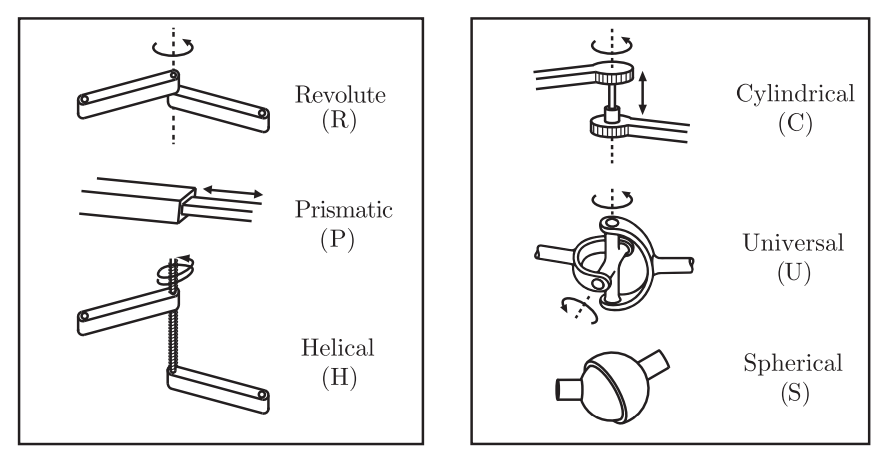
\includegraphics[width=0.8\linewidth]{image/robot_joints.png}
    \caption{Types of Robot Joint.}
    \label{fig:robot_joints}
\end{figure}

\hspace{1.27cm}
The aggregate degrees of freedom of a manipulator equals the sum of
the freedoms contributed by all its joints. A six-revolute-joint arm,
for example, possesses six independent DOF, giving its end-effector
the ability to reach any position and assume any orientation within
the reachable workspace, matching the mobility of a human arm. A
three-joint mechanism has a correspondingly simpler and more
constrained motion space, but this reduced complexity is often
advantageous in high-speed repetitive tasks such as pick-and-place.

%============================================================================
\subsection{Types of Manipulator Robot}

\subsubsection{Cartesian Manipulator Robots}
\hspace{1.27cm}
A Cartesian robot achieves end-effector motion exclusively through
independent linear translation along three mutually orthogonal axes,
each labelled $X$, $Y$, and $Z$ in correspondence with the standard
Cartesian coordinate system. Since each axis of motion is independent
and rectilinear, the kinematic equations governing the system are
relatively uncomplicated, making control system design and real-time
trajectory computation straightforward. This architecture excels in
applications requiring high geometric accuracy and excellent
repeatability, since positioning errors do not accumulate across
joints as they can in rotary-joint chains. The structural frame is
highly modular: standard aluminium extrusion and linear guide
profiles allow workspace volume to be scaled by adjusting the stroke
length of any axis. The rigidity of the gantry structure also
suppresses deflection and vibration when the robot operates over
large areas. Conversely, the rectilinear construction imposes
limitations: the end-effector cannot rotate, so wrist articulation
must be provided by supplementary mechanisms, and the machine
footprint grows in direct proportion to the required workspace
dimensions \autocite{sanchez-sanchez-2010}.\par
\begin{figure}[h]
    \centering
    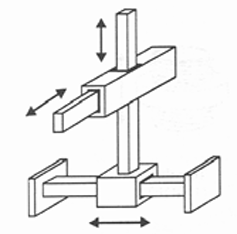
\includegraphics[width=0.5\linewidth]{image/cartesian.png}
    \caption{Cartesian Manipulator Robot.}
    \label{fig:cartesian_manipulator}
\end{figure}
\hspace{1.27cm}
Typical deployment environments for Cartesian robots include
automated assembly lines, computer numerical control (CNC) pick-and-
place machines, material handling gantries, and additive manufacturing
platforms such as 3D printers. Their combination of straightforward
control, scalable workspace, and high positional fidelity makes them
a practical choice wherever linear motion at speed and precision is
the dominant requirement.

%============================================================================
\subsubsection{Cylindrical Manipulator Robots}
\hspace{1.27cm}
A cylindrical manipulator defines its working volume in cylindrical
coordinates rather than Cartesian ones, producing a workspace that
resembles a hollow cylinder or annular region swept around a
vertical axis. The mechanical structure consists of three kinematic
elements: a revolute base joint that rotates the entire arm assembly
about the vertical axis, a prismatic joint that raises and lowers
the arm along that axis, and a second prismatic joint that extends
the arm radially outward or retracts it toward the axis. Together
these three joints provide access to any point within the
characteristic cylindrical shell without requiring the robot to
reorient its base.\par
\hspace{1.27cm}
This configuration offers several operational benefits:
\begin{itemize}
    \item A compact installation envelope suitable for tasks arranged
    around a central work area.
    \item The ability to combine angular sweep with independent linear
    extension, allowing workpieces at varying radial distances to be
    reached without reconfiguring the robot.
    \item Decoupled axis control that simplifies motion programming
    compared to fully rotary configurations.
\end{itemize}
The primary performance limitation is that the rotary base joint
introduces a degree of mechanical backlash that reduces end-effector
positioning accuracy relative to purely linear systems. Additionally,
the workspace does not extend to positions directly above the robot
base or to positions that require motion outside the defined
angular and radial limits, constraining the system's utility in
applications that demand full three-dimensional reachability
\autocite{10629493}.\par
\begin{figure}[h]
    \centering
    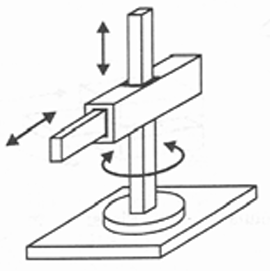
\includegraphics[width=0.5\linewidth]{image/cylindrical.png}
    \caption{Cylindrical Manipulator Robot.}
    \label{fig:cylindrical_manipulator}
\end{figure}
\hspace{1.27cm}
Industrial applications well matched to the cylindrical robot's
workspace geometry include loading and unloading machine tools,
transferring components between radially arranged workstations,
performing spot welds on circular weldments, and stacking items
vertically within a fixed horizontal footprint.

%============================================================================
\subsubsection{Spherical Manipulator Robots}
\hspace{1.27cm}
A spherical manipulator maps its motion capability onto spherical
coordinates, generating a workspace that approximates a partial
hollow sphere centred on the base. The kinematic chain comprises two
revolute joints, one providing rotation about the vertical base axis
and a second enabling vertical angular swing, together with a single
prismatic joint that telescopes the arm radially to adjust reach
distance. This arrangement allows the end-effector to be directed
toward nearly any point on the interior surface of the spherical
shell without requiring extensive base repositioning.\par
\hspace{1.27cm}
According to \autocite{1643416}, this architecture achieves a
favourable compromise between the volume of the accessible workspace
and the mechanical complexity of the structure. The capacity to swing
the arm vertically through a large arc makes spherical robots
particularly effective for tasks requiring access to positions above,
beside, or partially below the robot base, including operations
performed around large workpieces or through access openings. Compared
to Cartesian or cylindrical designs, the spherical robot provides
broader spatial coverage from a single mounting location, though at
the cost of more complex kinematic relationships that complicate
trajectory computation and limit the attainable absolute positioning
accuracy.\par
\begin{figure}[h]
    \centering
    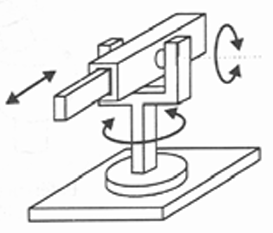
\includegraphics[width=0.5\linewidth]{image/spherical.png}
    \caption{Spherical Manipulator Robot.}
    \label{fig:spherical_manipulator}
\end{figure}
\hspace{1.27cm}
Spherical robots are predominantly deployed in applications where the
broad sweep of the workspace geometry provides operational value and
where end-effector orientation precision is a secondary requirement,
such as arc welding around large structural members, bulk material
transfer, die casting extraction, and machine tool tending.

%============================================================================
\subsubsection{Articulated Manipulator Robots}
\hspace{1.27cm}
Articulated manipulators are constructed as an open serial chain of
rigid links interconnected exclusively by revolute joints, producing
a kinematic topology that closely mirrors the anatomy of the human
upper limb. Commercial designs most commonly incorporate between four
and six such joints, with the six-joint variant providing full
six-degree-of-freedom control over both the position and orientation
of the end-effector. According to \autocite{parhi2012forward}, the
defining mechanical advantage of the articulated configuration is the
combination of a large reachable workspace with an ability to
approach any point within that workspace from multiple orientations,
a flexibility that exceeds what is achievable with Cartesian,
cylindrical, or spherical geometries. The ability to fold the arm
segments close to the body also allows the robot to reach into
confined spaces and around obstacles that would obstruct a less
agile mechanism.\par
\hspace{1.27cm}
These capabilities make articulated robots the configuration of
choice for tasks combining precise positioning with complex
tool-path control, including gas-metal arc welding, robotic painting,
precision component assembly, and camera-guided manipulation. The
technical challenges associated with articulated designs stem from
the nonlinear and coupled nature of the kinematic and dynamic
equations: inverse kinematics solutions are computationally
demanding, and errors in joint angle measurement or mechanical
backlash at any joint propagate through the chain and amplify at
the tip. Real-time compensation for these effects requires careful
attention to controller design and calibration.\par
\begin{figure}[h]
    \centering
    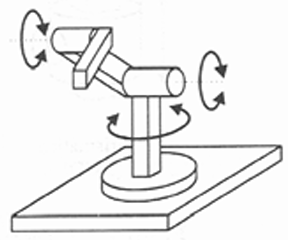
\includegraphics[width=0.5\linewidth]{image/articulated.png}
    \caption{Articulated Manipulator Robot.}
    \label{fig:articulated_manipulator}
\end{figure}
\hspace{1.27cm}
Articulated manipulators are in service across a broad spectrum of
manufacturing sectors, including automotive body-shop welding,
aerospace composite layup, consumer electronics assembly, and
pharmaceutical processing, wherever the simultaneous demand for a
large workspace, high positional accuracy, and flexible orientation
control justifies the investment in a more mechanically and
computationally complex platform.

%============================================================================
\subsubsection{SCARA Manipulator Robots}
\hspace{1.27cm}
The Selective Compliance Assembly Robot Arm, universally identified
by the acronym SCARA, was conceived by Professor Hiroshi Makino at
Yamanashi University during the early 1980s to address the specific
requirements of electronic component assembly: fast horizontal
positioning, precise vertical insertion, and controllable lateral
compliance. The mechanical architecture achieves these goals through
two horizontal revolute joints that sweep the arm through the $XY$
plane, a prismatic joint that drives the end-effector vertically,
and a fourth rotary axis at the wrist that sets tool orientation.
The selective compliance characteristic arises naturally from this
geometry: the arm is intentionally flexible in the horizontal plane,
allowing slight positional corrections during insertion tasks, but
rigid along the vertical $Z$-axis so that downward assembly forces
are resisted without deflection.
\begin{figure}[h]
    \centering
    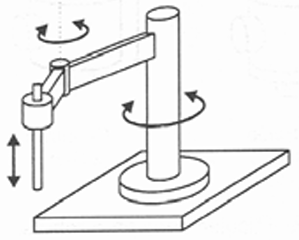
\includegraphics[width=0.5\linewidth]{image/scara.png}
    \caption{SCARA Manipulator Robot.}
    \label{fig:scara_manipulator}
\end{figure}
\par
\hspace{1.27cm}
In production environments SCARA robots are valued for their ability
to execute horizontal pick-and-place cycles at very high throughput.
Commercially available models achieve positional repeatabilities
within $\pm$0.01\,mm and complete single pick-place cycles in under
0.5\,seconds, performance figures that are difficult to match with
other configurations of comparable cost. Principal application domains
include printed circuit board population, pharmaceutical blister
pack loading, small component palletising, and in-process
dimensional inspection. In academic settings the SCARA architecture
is an effective vehicle for teaching kinematic analysis and motion
control because its relatively low degree-of-freedom count and
largely decoupled joint geometry simplify the derivation of both
forward and inverse kinematics solutions.

%============================================================================
\subsubsection{Parallel (Closed-Chain) Manipulator Robots}
\hspace{1.27cm}
A parallel manipulator departs from the conventional serial chain
architecture by connecting the end-effector to the fixed base through
multiple independent kinematic chains that operate simultaneously.
This closed-loop topology distributes the applied load across all
chains in parallel rather than concentrating it in the most distal
joint of a serial chain, producing a structure that is inherently
stiffer, exhibits lower moving inertia, and achieves a higher
ratio of payload capacity to total machine mass compared to
equivalent serial designs \autocite{merlet-2006}. The structural
stiffness of a closed kinematic loop is considerably greater than
that of an open chain of the same mass, and compliance-induced
positioning errors are both reduced in magnitude and more readily
detected and corrected \autocite{merlet-2006}. These mechanical
benefits are accompanied by a more restricted reachable workspace
and significantly more involved kinematic analysis than is required
for serial configurations \autocite{angeles-2004}.\par
\hspace{1.27cm}
A parallel robot may be formally described as a mechanism in which
an end-effector possessing $n$ degrees of freedom is coupled to a
fixed base through a minimum of two independent kinematic chains,
with exactly $n$ independently actuated joints distributed across
those chains \autocite{merlet-2006}. When the count of kinematic
chains equals exactly $n$, the mechanism is termed a fully parallel
manipulator. Three archetypal parallel configurations appear
repeatedly in the literature:
\begin{itemize}
    \item Stewart--Gough Platform: A six-degree-of-freedom
    fully parallel manipulator consisting of a rigid upper platform
    connected to a fixed base plate by six independently actuated
    telescoping struts, each terminating in universal and
    ball-and-socket joints. This architecture underpins the majority
    of six-axis motion simulators and ultra-precision machining
    platforms \autocite{merlet-2006}.
\begin{figure}[h]
    \centering
    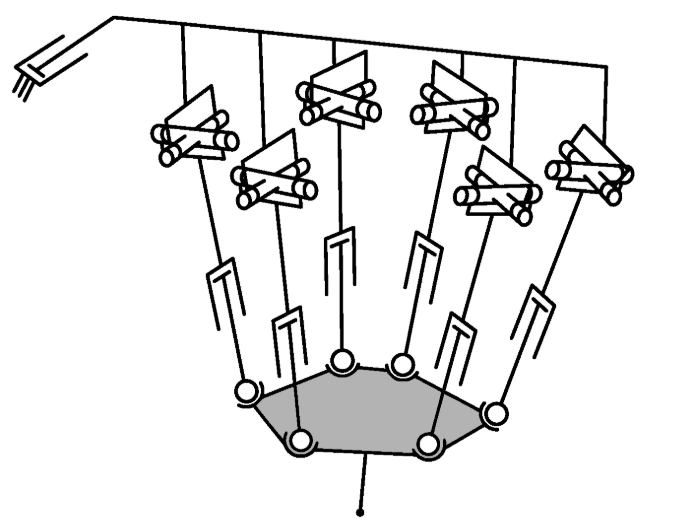
\includegraphics[width=0.5\linewidth]{image/Parallel6DOF.png}
    \caption{A 6-DOF Parallel Manipulator.}
    \label{fig:6DOF_parallel_manipulator}
\end{figure}
    \item Delta Robot: A three-degree-of-freedom
    translational parallel manipulator in which three kinematic
    chains restrict the moving platform to purely translational
    motion. Each chain combines a base-mounted rotary actuator with
    a passive parallelogram forearm. Because all actuators are
    located at the base, the moving mass is minimised, enabling
    cycle times below 0.3\,seconds and establishing this design as
    the standard platform for high-throughput pick-and-place in the
    food, pharmaceutical, and electronics industries
    \autocite{clavel-1990, merlet-2006}.
\end{itemize}
\begin{figure}[h]
    \centering
    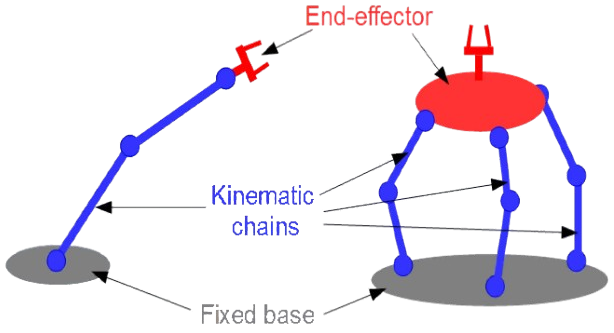
\includegraphics[width=0.5\linewidth]{image/Parallel.png}
    \caption{A 3-DOF Parallel Manipulator.}
    \label{fig:3DOF_Parallel}
\end{figure}

%============================================================================
\subsection{Delta Robot Kinematics}

\subsubsection{Geometric Description}
\hspace{1.27cm}
The geometry of a Delta robot is fully characterised by four
dimensional parameters: the side length $f$ of the equilateral
triangle formed by the fixed base joints, the side length $e$ of
the equilateral triangle formed by the moving platform joints,
the length $r_f$ of each proximal upper arm, and the length $r_e$
of each distal forearm \autocite{mzavatsky-2009}. Together these
four measurements determine the shape and volume of the reachable
workspace and govern the sensitivity of the end-effector position
to changes in joint angle. The origin of the reference coordinate
frame is located at the geometric centre of the fixed base triangle,
and the $z$-axis is directed downward so that every valid
end-effector position is assigned a negative $z$-coordinate.

\begin{figure}[h]
    \centering
    
\includegraphics[width=0.4\linewidth]{attachment3.png}
    \caption{Geometric parameters of the Delta robot: fixed base
             side $f$, moving platform side $e$, upper arm $r_f$,
             and forearm $r_e$ \autocite{mzavatsky-2009}.}
    \label{fig:delta_geometry}
\end{figure}

%============================================================================
\subsubsection{Forward Kinematics}
\hspace{1.27cm}
Forward kinematics (FK) addresses the problem of computing the
Cartesian end-effector position $(x_0, y_0, z_0)$ when the three
joint angles $(\theta_1, \theta_2, \theta_3)$ are known, for
example from encoder readings. For the Delta robot the solution
exploits the geometric interpretation of each forearm as the radius
of a sphere: the end-effector must lie simultaneously on three
spheres of radius $r_e$ centred at three adjusted joint positions
$J'_1$, $J'_2$, $J'_3$ derived from the joint angles
\autocite{zsombor-murray-2004}.\par
\hspace{1.27cm}
Pairwise subtraction of the three sphere equations cancels all
second-order terms in $x$ and $y$, leaving two equations that are
linear in the unknowns:

\begin{cequation}
    x_0 = a_1 z_0 + b_1, \qquad y_0 = a_2 z_0 + b_2
    \label{eq:fk_linear}
\end{cequation}

where the scalar coefficients $a_1,\, a_2,\, b_1,\, b_2$ depend
on the coordinates of the adjusted joint centres. Back-substituting
\autoref{eq:fk_linear} into one of the original sphere equations
produces a univariate quadratic equation in $z_0$:

\begin{multline}
    (a_1^2 + a_2^2 + 1)\,z_0^2
    \;+\; 2\bigl[a_1(b_1 - y_1) + a_2(b_2 - y_1) - z_1\bigr]\,z_0
    \;\\ + \; \bigl[(b_1 - y_1)^2 
    + (b_2 - y_1)^2 + z_1^2 -
    r_e^2\bigr] = 0
    \label{eq:fk_quadratic}
\end{multline}

Of the two roots of \autoref{eq:fk_quadratic} the physically
realizable configuration corresponds to the more negative value.
A negative discriminant signals that the supplied joint angles
cannot place the end-effector at any real point in space, indicating
a mechanically invalid configuration \autocite{mzavatsky-2009}. In
the system described in this thesis, FK is not used in the primary
motion-planning loop. Instead it functions as a post-movement
verification tool: after each commanded motion the encoder angles
are fed through FK and the computed position is compared against
the commanded target to identify gross mechanical faults.

%============================================================================
\subsubsection{Inverse Kinematics}
\hspace{1.27cm}
Inverse kinematics (IK) solves the complementary problem: given a
desired end-effector position $(x_0, y_0, z_0)$, find the joint
angle triplet $(\theta_1, \theta_2, \theta_3)$ that realises it.
The three-fold rotational symmetry of the Delta mechanism means
that each limb can be treated as an independent sub-problem
\autocite{mzavatsky-2009}. For the first limb the proximal joint is
mechanically constrained to rotate within the $YZ$ plane, reducing
the spatial three-sphere intersection to a two-circle intersection
problem in that plane.\par
\hspace{1.27cm}
The calculation begins by projecting the relevant end-effector
attachment point $E_1$ onto the $YZ$ plane to obtain $E'_1$. The
angular position of the proximal joint $J_1$ is then determined
as the intersection of a circle of radius $r_f$ centred on the
base attachment point $F_1$ with a circle of radius
$\sqrt{r_e^2 - x_0^2}$ centred on $E'_1$; where two intersections
exist, the geometrically admissible one is that with the smaller
$y$-coordinate. The corresponding joint angle follows from:

\begin{cequation}
    \theta_1 = \arctan\!\left(\frac{z_{J_1}}{y_{F_1} -
    y_{J_1}}\right)
    \label{eq:ik_theta1}
\end{cequation}

The second and third joint angles $\theta_2$ and $\theta_3$ are
computed by applying the same procedure to coordinate frames rotated
by $+120^{\circ}$ and $-120^{\circ}$ about the $Z$-axis
respectively \autocite{zsombor-murray-2004}. Should the
discriminant of the circle-intersection sub-problem be negative
for any limb, the requested position lies outside the reachable
workspace and the motion command must be rejected before any
actuation occurs.

%============================================================================
\subsection{Workspace Analysis}
\hspace{1.27cm}
The reachable workspace of a Delta robot encompasses all
end-effector positions that can be attained without any joint angle
exceeding its physical limit and without the mechanism passing
through a singular configuration. The outer boundary of this volume
approximates a cylinder whose top and bottom faces are bounded by
rounded surfaces determined by the geometric interference between
the kinematic chains. The specific shape and volume of the workspace
are governed primarily by the four geometric parameters $f$, $e$,
$r_f$, and $r_e$, with the actuator joint-angle limits providing
the secondary constraint \autocite{stock-2003}.\par
\hspace{1.27cm}
Accurate workspace knowledge serves two practical purposes in the
present system. First, it establishes the set of robot-frame
coordinates for which the IK solver will return a valid solution;
any object position reported by the vision system that falls outside
this region must be discarded by the safety module before it can
be forwarded to the motion controller. Second, the workspace
boundary provides the spatial reference needed to position the
RealSense D455 camera so that its field of view completely
encompasses the area within which objects can be picked
\autocite{bonev-2001}.

\begin{figure}[h]
    \centering
    \includegraphics[width=0.7\linewidth]{image/Reachable workspace
    of a Delta robot.jpg}
    \caption{Reachable workspace of a Delta robot, approximating a
             cylindrical volume \autocite{stock-2003}.}
    \label{fig:workspace_delta}
\end{figure}

%============================================================================
\subsection{Vision System: Camera and 2D Localisation}

\subsubsection{Intel RealSense D455}
\hspace{1.27cm}
The Intel RealSense D455 is a structured-light stereo camera that
combines a passive infrared stereo imager pair with an active
infrared flood illuminator and a co-located colour sensor. Its
stereo baseline of 95\,mm exceeds that of the D435 model (55\,mm),
providing more stable image acquisition at the operating distance
used in this system \autocite{intel-realsense-d455}. The colour
stream delivers up to 30\,frames per second at resolutions suitable
for real-time object detection, and the associated intrinsic
calibration data including focal lengths $f_x$, $f_y$ and
principal-point coordinates $c_x$, $c_y$ are published
continuously on the \texttt{camera\_info} topic within the ROS~2
graph.

\subsubsection{Pinhole Camera Model}
\hspace{1.27cm}
The imaging geometry of the RealSense D455 colour sensor is
modelled by the standard pinhole projection. A physical point
$\mathbf{P}_c = [X_c,\, Y_c,\, Z_c]^{\top}$ in the camera
coordinate frame projects onto the image plane at pixel
coordinates $(u, v)$ according to \autocite{hartley-2004}:

\begin{cequation}
    \begin{bmatrix} u \\ v \\ 1 \end{bmatrix}
    =
    \frac{1}{Z_c}
    \begin{bmatrix}
        f_x & 0   & c_x \\
        0   & f_y & c_y \\
        0   & 0   & 1
    \end{bmatrix}
    \begin{bmatrix} X_c \\ Y_c \\ Z_c \end{bmatrix}
    =
    \frac{1}{Z_c}\, \mathbf{K}\, \mathbf{P}_c,
    \label{eq:pinhole_matrix}
\end{cequation}

where $\mathbf{K}$ is the $3 \times 3$ camera intrinsic matrix.
Expanding \autoref{eq:pinhole_matrix} gives the familiar
component-wise projection equations:

\begin{cequation}
    u = f_x \cdot \frac{X_c}{Z_c} + c_x,
    \qquad
    v = f_y \cdot \frac{Y_c}{Z_c} + c_y.
    \label{eq:pinhole_uv}
\end{cequation}

The four intrinsic parameters are defined as follows:
$f_x = f / s_x$ and $f_y = f / s_y$, where $f$ is the physical
focal length of the lens and $s_x$, $s_y$ are the horizontal and
vertical pixel pitch of the image sensor; $c_x$ and $c_y$ are the
coordinates of the principal point, ideally located at the image
centre but offset by small manufacturing tolerances.

\subsubsection{2D Localisation via Fixed-Height Backprojection}
\hspace{1.27cm}
Since every target object in this system rests on the conveyor
belt surface at a fixed, pre-measured height below the camera,
the scene depth is not unknown but constant: $Z_c = Z_{\text{belt}}$
for all objects. This constraint eliminates the need for per-frame
depth measurement and allows the full pixel-to-camera-frame
localisation to be performed using only the colour image.

\par
\hspace{1.27cm}
Inverting \autoref{eq:pinhole_uv} under the fixed-depth
assumption yields the camera-frame planar coordinates of a
detected object directly from its pixel centre $(u, v)$:

\begin{cequation}
    X_c = \frac{(u - c_x)\cdot Z_{\text{belt}}}{f_x},
    \qquad
    Y_c = \frac{(v - c_y)\cdot Z_{\text{belt}}}{f_y}.
    \label{eq:backproject}
\end{cequation}

In homogeneous matrix notation, this backprojection can be
written as:

\begin{cequation}
    \begin{bmatrix} X_c \\ Y_c \\ Z_c \end{bmatrix}
    =
    Z_{\text{belt}}\,
    \mathbf{K}^{-1}
    \begin{bmatrix} u \\ v \\ 1 \end{bmatrix}
    =
    Z_{\text{belt}}
    \begin{bmatrix}
        \frac{1}{f_x} & 0              & -\frac{c_x}{f_x} \\[4pt]
        0              & \frac{1}{f_y} & -\frac{c_y}{f_y} \\[4pt]
        0              & 0              & 1
    \end{bmatrix}
    \begin{bmatrix} u \\ v \\ 1 \end{bmatrix}.
    \label{eq:backproject_matrix}
\end{cequation}

The scalar $Z_{\text{belt}}$ is determined once during system
setup as the physically measured vertical distance from the camera
optical centre to the belt surface, and it remains constant
throughout operation. The resulting 3D point
$[X_c,\, Y_c,\, Z_{\text{belt}}]^{\top}$ expressed in the camera
frame is then forwarded to the coordinate frame transformation
stage described in \autoref{sec:coordinate_transform}.

\subsubsection{Intrinsic Parameter Acquisition}
\hspace{1.27cm}
The four intrinsic parameters $f_x$, $f_y$, $c_x$, $c_y$ required
by \autoref{eq:pinhole_matrix} are not hardcoded but are read at
runtime from the \texttt{/camera/color/camera\_info} topic
published by the \texttt{realsense2\_camera} ROS~2 node. The
\texttt{camera\_info} message carries the full $3 \times 3$ intrinsic
matrix $\mathbf{K}$ as a row-major nine-element array. In the
detection node, the parameters are extracted on the first message
receipt and cached for the remainder of the session:

\begin{cequation}
    \mathbf{K} =
    \begin{bmatrix}
        K[0] & 0    & K[2] \\
        0    & K[4] & K[5] \\
        0    & 0    & 1
    \end{bmatrix}
    =
    \begin{bmatrix}
        f_x & 0   & c_x \\
        0   & f_y & c_y \\
        0   & 0   & 1
    \end{bmatrix}.
    \label{eq:K_from_topic}
\end{cequation}

Reading $\mathbf{K}$ from the live topic rather than a static
configuration file ensures that the correct parameters are used
regardless of any change in camera resolution or mounting, since
the RealSense driver recomputes and publishes the intrinsics
appropriate to the active stream profile on every startup.

%============================================================================
\subsection{Coordinate Frame Transformation}
\hspace{1.27cm}
Once the image-plane position of a detected object has been
determined, it must be expressed in the robot base frame before
it can serve as an input to the inverse kinematics solver. This
mapping is a rigid-body transformation — commonly referred to
as hand-eye calibration — that encodes the fixed geometric
relationship between the camera coordinate frame and the robot
base frame. The general form of the transformation is a
homogeneous matrix $\mathbf{H}$ comprising a $3 \times 3$
rotation matrix $\mathbf{R}$ and a $3 \times 1$ translation
vector $\mathbf{T}$:

\begin{cequation}
    \mathbf{H} =
    \begin{bmatrix}
        \mathbf{R} & \mathbf{T} \\
        \mathbf{0}^{\top} & 1
    \end{bmatrix},
    \label{eq:homogeneous}
\end{cequation}

so that a point $\mathbf{p}_c = [X_c,\, Y_c,\, Z_c,\, 1]^{\top}$
expressed in the camera frame is mapped to the robot base frame
as:

\begin{cequation}
    \begin{bmatrix} X_r \\ Y_r \\ Z_r \\ 1 \end{bmatrix}
    =
    \begin{bmatrix}
        \mathbf{R} & \mathbf{T} \\
        \mathbf{0}^{\top} & 1
    \end{bmatrix}
    \begin{bmatrix} X_c \\ Y_c \\ Z_c \\ 1 \end{bmatrix}
    =
    \mathbf{R}
    \begin{bmatrix} X_c \\ Y_c \\ Z_c \end{bmatrix}
    + \mathbf{T}.
    \label{eq:transform}
\end{cequation}

\hspace{1.27cm}
The rotation matrix $\mathbf{R}$ is a $3 \times 3$ orthonormal
matrix of the first kind ($\det(\mathbf{R}) = 1$) that encodes
the angular orientation of the camera frame relative to the robot
base frame. Any such rotation can be parameterised by a unit
axis vector $\hat{n} = [n_1,\, n_2,\, n_3]^{\top}$ and a
rotation angle $\theta$ through the Rodrigues formula
\autocite{tsai-lenz-1989}:

\begin{multline}
    \mathbf{R} =
    \begin{bmatrix}
        n_1^2 + (1-n_1^2)\cos\theta &
        n_1 n_2(1-\cos\theta) - n_3\sin\theta &
        n_1 n_3(1-\cos\theta) + n_2\sin\theta \\[4pt]
        n_1 n_2(1-\cos\theta) + n_3\sin\theta &
        n_2^2 + (1-n_2^2)\cos\theta &
        n_2 n_3(1-\cos\theta) - n_1\sin\theta \\[4pt]
        n_1 n_3(1-\cos\theta) - n_2\sin\theta &
        n_2 n_3(1-\cos\theta) + n_1\sin\theta &
        n_3^2 + (1-n_3^2)\cos\theta
    \end{bmatrix}.
    \label{eq:rodrigues}
\end{multline}

The translation vector $\mathbf{T} = [t_x,\, t_y,\, t_z]^{\top}$
encodes the position of the camera optical centre expressed in
the robot base frame, accounting for the physical mounting offset
of the camera relative to the robot origin.

\subsubsection{Coordinate Frame Definitions}
\hspace{1.27cm}
Following the notation of \autocite{tsai-lenz-1989}, four
coordinate frames are relevant to the transformation:

\begin{itemize}
    \item $\mathcal{F}_r$ : the robot base frame,
    fixed at the kinematic origin of the robot. All motor commands
    and IK inputs are expressed in this frame.
    \item $\mathcal{F}_c$ : the camera frame, centred
    at the camera optical centre with the $z$-axis coinciding
    with the optical axis and the $x$- and $y$-axes aligned with
    the image plane horizontal and vertical directions,
    respectively.
    \item $\mathcal{F}_w$ : the calibration world frame,
    an auxiliary frame defined on the calibration target at known
    positions during the calibration procedure.
    \item $\mathcal{F}_b$ : the belt (object) frame,
    the plane in which detected objects reside, at a fixed and
    measured height $Z_{\text{fixed}}$ below $\mathcal{F}_r$.
\end{itemize}

\subsubsection{Calibration Procedure}
\hspace{1.27cm}
The process of determining $\mathbf{R}$ and $\mathbf{T}$ is
known as \textit{eye-to-hand calibration} when the camera is
mounted at a fixed location in the workspace rather than on the
robot arm. Tsai and Lenz \autocite{tsai-lenz-1989} showed that
this relationship can be recovered from a set of corresponding
point observations without requiring global nonlinear
optimisation: the problem decomposes into first solving for the
rotation $\mathbf{R}$ via a linear least-squares system, and
subsequently solving for the translation $\mathbf{T}$ from a
second linear system given the already-determined $\mathbf{R}$.
The minimum number of calibration stations required for a unique
solution is three \autocite{tsai-lenz-1989}.

\par
\hspace{1.27cm}
In this system, an empirical axis-alignment calibration procedure
is adopted, following the physical verification approach. The
procedure is carried out in four sequential steps:

\begin{enumerate}
    \item Origin alignment: A reference object is placed
    at the geometric centre of the robot workspace, where
    $X_r \approx 0$ and $Y_r \approx 0$ by definition. The
    translation offsets $t_x$ and $t_y$ in $\mathbf{T}$ are
    adjusted until the reported robot-frame coordinates of the
    detected object match the known physical position.

    \item Axis sign and assignment verification: The
    object is displaced in the positive $X_r$ direction by a
    known distance $\Delta x$. If the reported coordinate
    increases accordingly, the $X$ axis mapping is confirmed.
    If it decreases, the sign of the corresponding column of
    $\mathbf{R}$ is negated. The same test is repeated for the
    $Y_r$ direction.

    \item Scale validation: The object is moved to a
    set of positions at known metric distances from the origin.
    The Euclidean error between the reported and measured
    positions is computed. If errors exceed the acceptable
    threshold, the focal-length and principal-point parameters
    used in the projection are re-verified against the live
    \texttt{camera\_info} topic.

    \item Full-workspace validation: The object is
    placed at five or more positions distributed across the
    robot workspace. The mean and maximum absolute errors in
    $X_r$ and $Y_r$ are recorded. Calibration is accepted when
    the mean error is below 5\,mm across all test positions.
\end{enumerate}

\subsubsection{Transformation Matrix Construction}
\hspace{1.27cm}
For the fixed eye-to-hand mounting geometry used in this system,
the camera is positioned above the workspace with its optical
axis directed downward and slightly offset from the robot
base-frame origin. The rotation matrix $\mathbf{R}$ encodes two
effects: the physical angular mounting of the camera (roll,
pitch, yaw relative to the robot frame) and the axis convention
difference between the camera frame (where $y$ points downward
in the image) and the robot frame (where $Y$ points in the
robot's forward direction). In practice, $\mathbf{R}$ takes the
form of a sign-permutation matrix with possible negations,
determined through the axis verification procedure described
above. Once the calibration is complete, the full transformation
from a detected pixel centre $(u, v)$ to robot base-frame
coordinates $(X_r, Y_r)$ is:

\begin{cequation}
    \begin{bmatrix} X_r \\ Y_r \end{bmatrix}
    =
    \mathbf{R}_{2 \times 2}
    \begin{bmatrix} X_c \\ Y_c \end{bmatrix}
    +
    \begin{bmatrix} t_x \\ t_y \end{bmatrix},
    \label{eq:transform_2d}
\end{cequation}

where $X_c$ and $Y_c$ are the camera-frame coordinates derived
from the pixel observation and the known belt height
$Z_{\text{fixed}}$, and $\mathbf{R}_{2 \times 2}$ is the
upper-left $2 \times 2$ submatrix of $\mathbf{R}$ applicable to
the planar constraint. The vertical robot coordinate $Z_r$ is
not computed from the camera but is set to the fixed pick height
$Z_{\text{pick}}$ measured during system setup, consistent with
the flat-world assumption that all target objects rest on the
belt surface at a constant elevation.

%============================================================================
\subsection{Object Detection: YOLO}
\hspace{1.27cm}
You Only Look Once (YOLO) refers to a line of single-stage
convolutional neural network architectures in which object
detection is formulated as a direct regression from the input
image to a set of bounding box parameters and class probability
vectors, with the entire computation performed in a single
forward pass through the network \autocite{redmon-2016}. By
eliminating the region-proposal stage that is characteristic of
two-stage detectors such as Faster R-CNN, YOLO achieves inference
latencies that are well suited to closed-loop robotic systems
where the speed of the detection result directly limits the
achievable control bandwidth.

\begin{figure}[h]
    \centering
    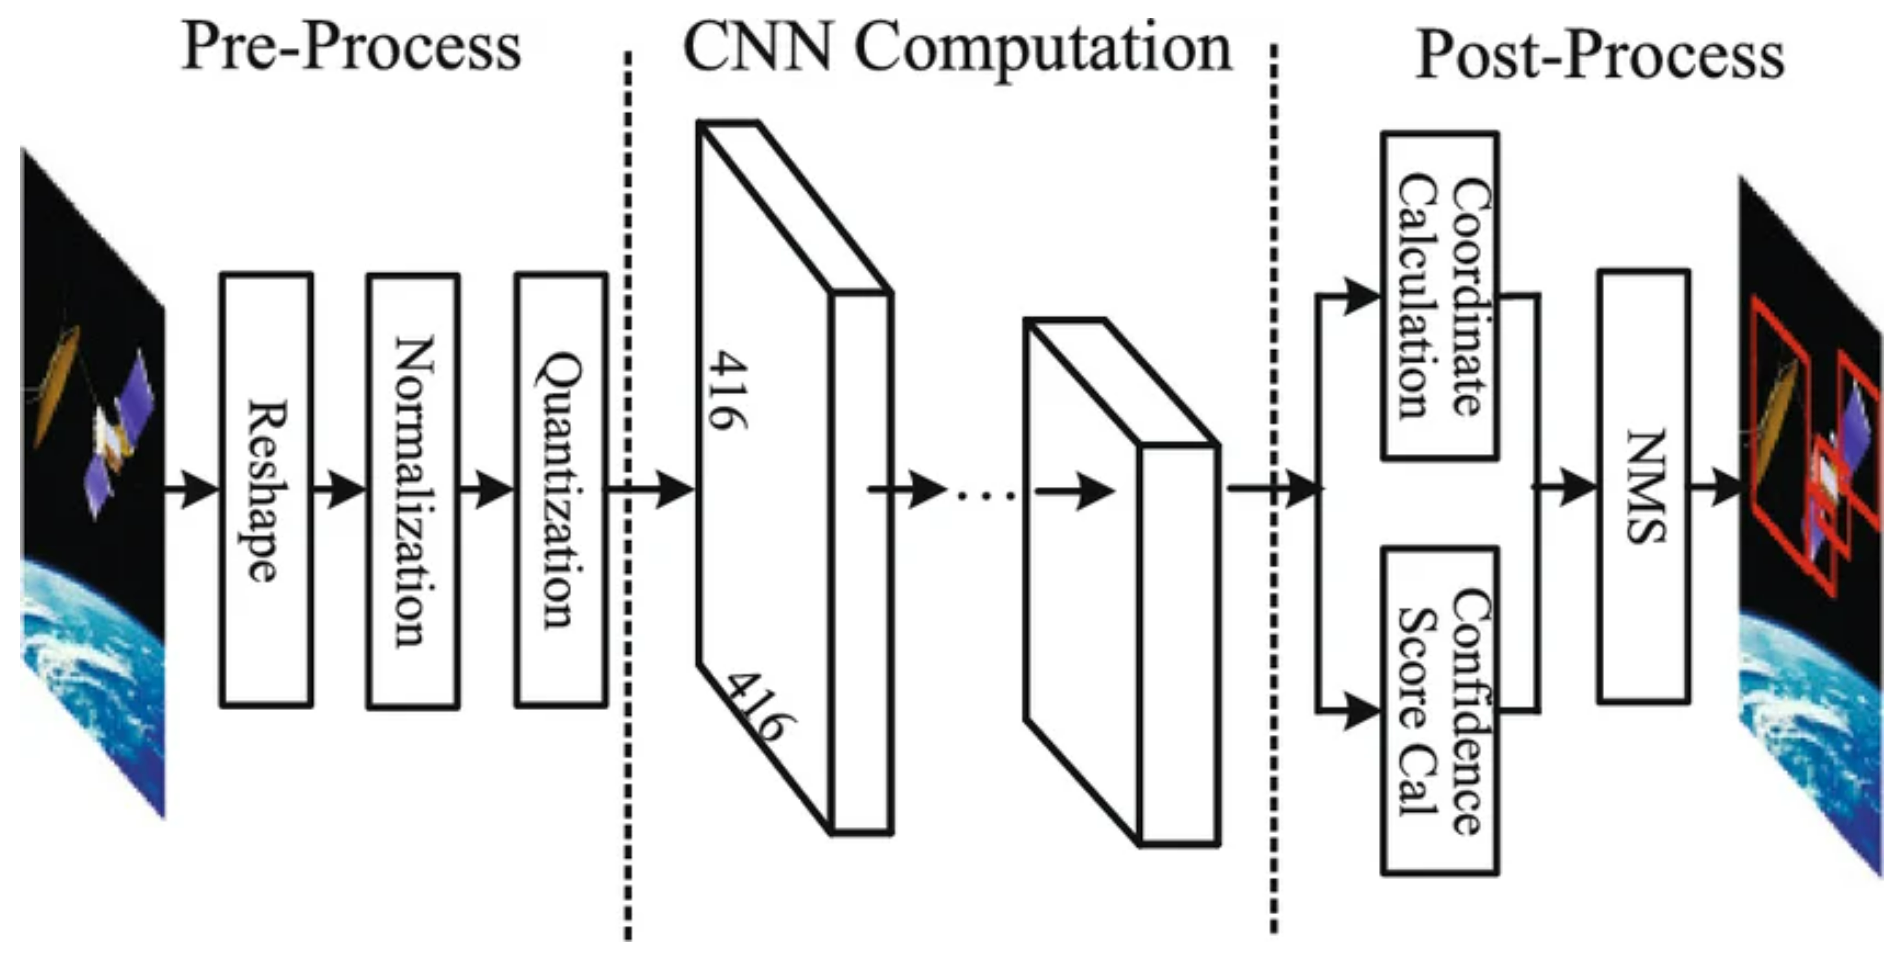
\includegraphics[width=0.7\linewidth]{image/Architecture of the YOLO network.png}
    \caption{Architecture of The YOLO Network \autocite{redmon-2016}.}
    \label{fig:YOLO architecure}
\end{figure}



\par
\hspace{1.27cm}
The family has evolved through multiple generations, from the
original network through YOLOv5, YOLOv7, YOLOv8, and the YOLO11
series, each introducing architectural refinements that improve
the precision-recall curve and reduce inference time on embedded
GPU hardware \autocite{jocher-2023}. In pick-and-place
applications, the centroid $(u, v)$ of the bounding box returned
by the detector is taken as the pixel-plane position of the
target object and forwarded to the coordinate transformation
stage.

%============================================================================
\subsection{Trajectory Planning and Control}
\hspace{1.27cm}
Trajectory planning is the process of computing a
time-parameterised sequence of end-effector positions,
velocities, and accelerations that connects an initial
configuration to a goal configuration while simultaneously
satisfying the velocity, acceleration, and jerk constraints
imposed by the physical actuators and the structural dynamics
of the mechanism \autocite{biagiotti-2008}. For Delta robots,
where the moving platform is extremely lightweight and the
parallel linkages exhibit low structural damping, trajectory
quality has a direct and measurable effect on placement
accuracy: a poorly shaped motion profile excites the natural
resonance modes of the linkage structure, producing residual
oscillations at the end-effector that persist after the
nominal motion has ended and degrade pick-and-place
repeatability \autocite{siciliano-2009}.

\subsubsection{Joint-Space and Cartesian-Space Planning}
\hspace{1.27cm}
Trajectory planning for robotic manipulators can be performed
either in joint space or in Cartesian space, and the choice
has practical consequences for path predictability and
computational load \autocite{siciliano-2009}. In
joint-space planning, a smooth scalar function
$\theta_i(t)$ is constructed independently for each joint
angle between its initial and final values. The resulting
end-effector path in Cartesian space is not a straight line
but follows whatever curve the forward kinematics maps the
joint interpolation onto. However, joint-space planning
guarantees that velocity and acceleration limits are satisfied
by construction and avoids continuous IK evaluations during
motion execution. In Cartesian-space planning, the
desired end-effector position
$\mathbf{p}(t) = [x(t),\, y(t),\, z(t)]^{\top}$ is defined
directly as a function of time, and the IK solver is invoked
at every control step to convert the Cartesian setpoint to
joint coordinates. This approach produces geometrically
predictable straight-line or curved paths at the cost of
continuous IK computation and increased risk of encountering
workspace boundaries or kinematic singularities mid-trajectory
\autocite{biagiotti-2008}.

\subsubsection{Polynomial Velocity Profiles}
\hspace{1.27cm}
Regardless of whether planning is performed in joint space or
Cartesian space, a time-scaling function $s(t)$ is used to
shape the velocity and acceleration profiles of each motion
segment. Two profile forms are widely used in the robotics
literature \autocite{biagiotti-2008}.

\par
\hspace{1.27cm}
\begin{itemize}
    \item Trapezoidal profile is divided into three phases, a constant-acceleration phase of duration $t_a$, a
constant-velocity cruise phase, and a symmetric
constant-deceleration phase. The velocity profile is:
\end{itemize}


\begin{cequation}
    \dot{s}(t) =
    \begin{cases}
        \dfrac{v_{\max}}{t_a}\, t,
            & 0 \leq t < t_a \\[6pt]
        v_{\max},
            & t_a \leq t \leq T - t_a \\[6pt]
        \dfrac{v_{\max}}{t_a}(T - t),
            & T - t_a < t \leq T
    \end{cases}
    \label{eq:trap_vel}
\end{cequation}

where $v_{\max}$ is the peak velocity and $T$ is the total
segment duration. The acceleration is piecewise constant at
$\pm v_{\max}/t_a$, meaning the jerk at the phase transition
points is theoretically unbounded. For high-speed lightweight
mechanisms such as Delta robots, this jerk discontinuity
excites structural resonance and causes residual vibration at
the end-effector \autocite{siciliano-2009}.

\par
\hspace{1.27cm}
\begin{itemize}
\item Quintic polynomial profile is a degree-five polynomial
satisfying boundary conditions of zero displacement error,
zero velocity, and zero acceleration at both the start and
end of the segment provides continuity through the second
derivative, eliminating the jerk discontinuity of the
trapezoidal profile \autocite{biagiotti-2008}. Using the
normalised time variable $\tau = t/T \in [0, 1]$, the profile
is:
\end{itemize}
\begin{cequation}
    s(\tau) = 10\tau^3 - 15\tau^4 + 6\tau^5,
    \label{eq:quintic}
\end{cequation}

with velocity and acceleration:

\begin{cequation}
    \dot{s}(\tau) = \frac{1}{T}
    \left(30\tau^2 - 60\tau^3 + 30\tau^4\right),
    \label{eq:quintic_vel}
\end{cequation}

\begin{cequation}
    \ddot{s}(\tau) = \frac{1}{T^2}
    \left(60\tau - 180\tau^2 + 120\tau^3\right).
    \label{eq:quintic_acc}
\end{cequation}

The smooth bell-shaped velocity profile and the continuous
acceleration curve of
\autoref{eq:quintic}--\autoref{eq:quintic_acc} suppress
structural excitation and make the quintic polynomial the
preferred time-scaling function for lightweight parallel
manipulators where residual vibration is the dominant source
of placement error \autocite{biagiotti-2008}.

\subsubsection{Actuator-Level Control}
\hspace{1.27cm}
At the actuator level, modern brushless servo motors and
quasi-direct-drive (QDD) actuators typically implement an
onboard PD position controller that closes the position loop
at high frequency independently of the host computer. The
general form of the torque command is \autocite{siciliano-2009}:

\begin{cequation}
    \tau = K_p\,(\theta_{\text{des}} - \theta_{\text{enc}})
         + K_d\,(\dot{\theta}_{\text{des}} -
         \dot{\theta}_{\text{enc}}),
    \label{eq:pd_control}
\end{cequation}

where $\tau$ is the output torque, $\theta_{\text{des}}$ and
$\dot{\theta}_{\text{des}}$ are the desired position and
velocity set-points, $\theta_{\text{enc}}$ and
$\dot{\theta}_{\text{enc}}$ are the encoder-measured position
and velocity, and $K_p$, $K_d$ are the proportional and
derivative gains. When this local control loop is combined with
a supervisory Cartesian trajectory planner operating in
real-time, the overall architecture separates motion shaping
from position regulation: the planner is responsible for
producing smooth, dynamically feasible set-points, while the
onboard controller is responsible for tracking those set-points
accurately despite actuator dynamics and disturbances
\autocite{siciliano-2009}.

\subsubsection{Forward Kinematics Validation}
\hspace{1.27cm}
In closed-loop motion control of parallel robots, it is
standard practice to verify the actual end-effector position
after each commanded motion by reading the joint encoder values
and applying the forward kinematics model \autocite{merlet-2006}.
This post-motion validation step detects discrepancies between
the commanded and achieved positions that may result from
mechanical compliance, actuator saturation, or CAN communication
faults. If the Euclidean error between the FK-computed position
and the commanded target exceeds a defined threshold, the
controller can halt the motion sequence, trigger a fault
response, and return the robot to a safe home position before
the next pick cycle begins. This validation approach is
particularly important in vision-guided systems, where an
uncorrected positioning error in one cycle can compound with
a subsequent detection error in the next \autocite{yamtuan-2023}.

%============================================================================
\subsection{Pick-and-Place Operation}
\hspace{1.27cm}
Pick-and-place represents the core operational sequence for which
the Delta robot was originally designed and remains its dominant
industrial application \autocite{biagiotti-2008}. A complete
cycle is decomposed into four sequential motion phases, each
defined by a set of Cartesian waypoints:

\begin{enumerate}
    \item Approach: Starting from the home configuration,
    the end-effector travels horizontally to a position vertically
    above the target object while maintaining a safety clearance
    height that prevents any contact with the work surface.

    \item Descend and Grasp: The end-effector descends
    vertically to the object surface elevation and the gripper
    (pneumatic suction cup or mechanical jaw) is actuated to
    secure the object.

    \item Lift and Transfer: The end-effector retracts
    vertically to the safety clearance height with the object
    held securely, then translates horizontally to the designated
    placement location along a smoothly profiled trajectory.

    \item Place and Release: The end-effector descends
    to the placement elevation, the gripper releases, and the
    robot returns to the home position in preparation for the
    next detection cycle.
\end{enumerate}

\hspace{1.27cm}
Each Cartesian waypoint in the above sequence is individually
validated by the IK solver before execution begins. Any waypoint
that maps to a configuration outside the reachable workspace
triggers an immediate abort, returning the robot to the home
position without attempting the motion \autocite{yamtuan-2023}.

%============================================================================
\subsection{Key Control and Software}

\subsubsection{Robot Operating System 2 (ROS~2)}
\hspace{1.27cm}
ROS~2 is an open-source distributed robotics middleware framework
developed as a ground-up redesign of the original ROS~1
infrastructure, addressing limitations that became apparent as
ROS~1 was deployed in safety-critical and multi-robot industrial
applications \autocite{ros2-2022}. The most significant
architectural departure from its predecessor is the adoption of
the Data Distribution Service (DDS) standard as the underlying
communication layer. DDS provides a fully decentralised,
broker-free publish-subscribe transport that supports deterministic
delivery guarantees, configurable Quality of Service (QoS) policies
for controlling message priority, reliability, and latency, and
native inter-process as well as intra-process communication
without requiring a central master process.\par
\begin{figure}[h]
    \centering
    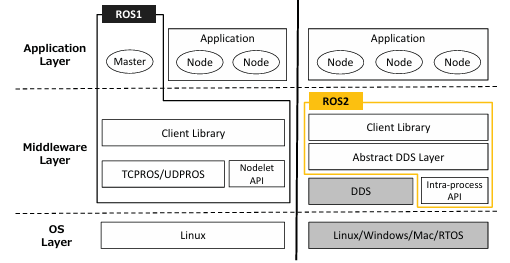
\includegraphics[width=0.7\linewidth]{image/ros2 art.png}
    \caption{ROS~2 Layered Software Architecture.}
    \label{fig:ROS2_Architecture}
\end{figure}
\hspace{1.27cm}
The layered structure of ROS~2, shown in
\textbf{\autoref{fig:ROS2_Architecture}}, positions user
application nodes at the top tier. Developers write these nodes
in C++ using the \texttt{rclcpp} client library or in Python using
\texttt{rclpy}, both of which expose an identical set of
communication primitives so that subsystems written in different
languages can interoperate transparently. These client libraries
issue calls to an abstract DDS interface layer that insulates
application code from the specifics of the DDS vendor in use,
and below this layer the chosen DDS implementation handles
all message serialisation, transport, and delivery. The lowest
tier is the host operating system; ROS~2 runs on Linux, Windows,
and macOS, and a real-time profile enables deployment on RTOS
kernels where deterministic scheduling latency is required.

%============================================================================
\subsubsection{CAN Bus}
\hspace{1.27cm}
The Controller Area Network (CAN) protocol is a differential-pair
serial bus standard originally developed by Bosch for use in
automotive electronic control systems and subsequently adopted
as the preferred intra-machine communication medium for industrial
robot drives \autocite{bosch-can-1991}. Its appeal in robotics
applications derives from a combination of high noise immunity on
the differential signal pair, non-destructive bitwise
priority-based bus arbitration that avoids data collisions, and
deterministic message latency at data rates of up to 1\,Mbit/s
for classic CAN or up to 8\,Mbit/s for the newer CAN~FD variant.
These properties allow motor controllers distributed around the
robot arm to be polled and updated at rates of several hundred
hertz over a single two-wire cable.\par

\begin{figure}[h]
    \centering
    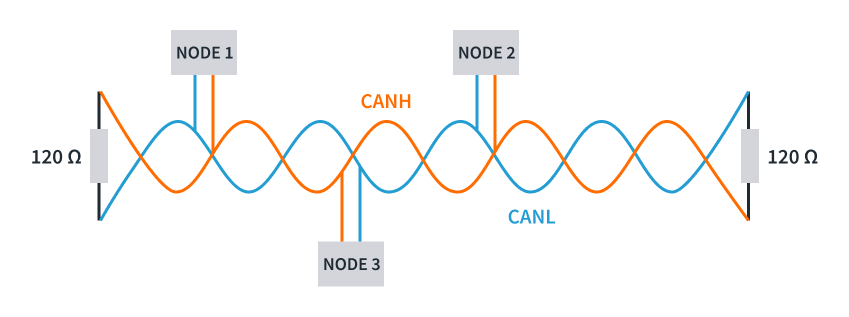
\includegraphics[width=0.8\linewidth]{image/interface-can-bus.png}
    \caption{Hardware Interface of CAN Bus.}
    \label{fig:CAN Bus}
\end{figure}

%============================================================================
% END OF CHAPTER 2
%============================================================================
